\documentclass[12pt,a4paper]{article}

\usepackage{cite} % Add this line to include the cite package
% \usepackage[backref]{hyperref} % Add this line to include the hyperref package

\usepackage{lmodern}
\usepackage{fix-cm}
\usepackage{ctex} % Add this line to include the ctex package
\usepackage{amsmath} % Add this line to include the amsmath package
\usepackage{graphicx} % Add this line to include the graphicx package
\usepackage{fancyhdr}

\title{\textbf{Answer}}
\author{Author: Pan Changxun}
\date{}
%\date{April 2025}

\topmargin=-0.45in      %
\evensidemargin=0in     %
\oddsidemargin=0in      %
\textwidth=6.5in   
\textheight=9.0in       %
\headsep=0.25in 
\setlength{\headheight}{15pt}  % Increased to fix fancyhdr error

\pagestyle{fancy}
\fancyhf{} % Clear all header and footer fields
\fancyhead[L]{Ciallo\(\sim( \cdot\ \omega\) <} % Left header
\fancyhead[C]{物竞模拟卷} % Center header
\fancyhead[R]{test} % Right header
%\fancyfoot[L]{\leftmark} % Left footer
\fancyfoot[C]{\thepage} % Center footer
%\fancyfoot[R]{} % Right footer

\begin{document}
\maketitle
\footnotesize

\section{Chainball (60pts)}
如图\ref{fig:chainball} 所示,一个简单的链条球模型由三个质量为$m$的球体和两根无质量的轻绳组成。现在固定最上方的一个球体,并自然下垂。绳子的长度均为\(l\), 重力加速度为\(g\).

\begin{figure}[htbp]
	\centering
	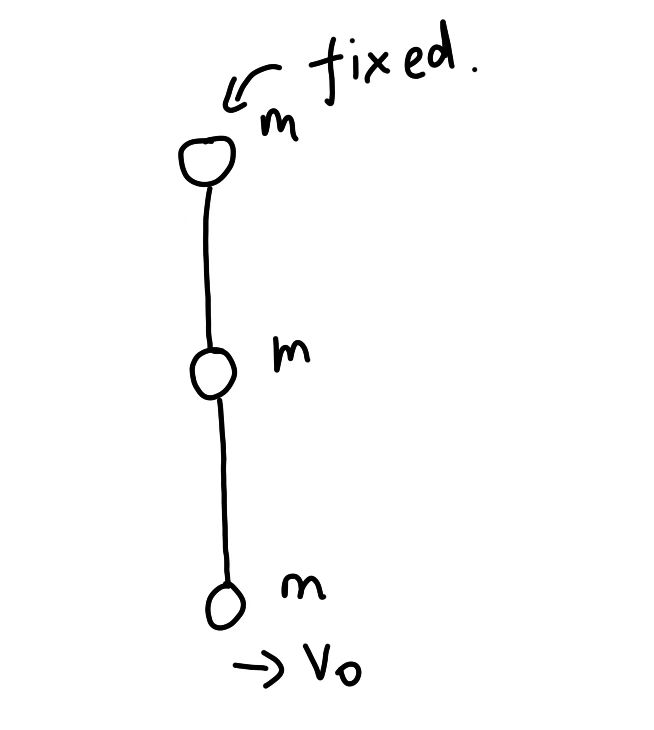
\includegraphics[width=0.3\textwidth]{chainball}
	\caption{三个质量为$m$的球体由两根无质量的轻绳连接成链条球模型,最上方的球体固定.}
	\label{fig:chainball}
\end{figure}

\begin{enumerate}
	\item 现在突然给予最下方的球体一个向右的初速度$v_0$,求出最下方球体的水平方向上的位移随时间变化的关系式。(设\(v_{0}\)很小可以视为小振动)(30pts)
	\item 在第一小问的设定下,最下方球体水平方向上最远可以达到的位移是多少?(4pts)
	\item 现在只限制下方小球的初速度为向右的初速度为\(v_0\),请问是否有方式使得摆动看起来“更有规律”?即:每次当中间球体回到最低点时,最下方的球体也回到最低点。如果有,请给出所有还需要的条件;如果没有,请给出理由。(16ps)
	\item 下面考虑一个更复杂一点的情况:现在由\(n+2\)个质量为\(m\)的球体组成类似的链条球模型。如图\ref{fig:chainball2}所示。为了更容易计算,现设定如下:初始时上方\(n\)个球均是固定的,只有最下方两个球可以自由移动,仍然给予最下方球初速度\(v_{0}\),当倒数第二个球体再次回到最低点的时刻,通过Teyvat的神秘力量使得最后一根绳子断裂(即编号为0的球体会脱落),同时解除编号为2的球体的锁定。如此递推,每次保持只有两个球体会活动,直到只剩下编号为\(n\)与\(n+1\)的球体。请求出此时编号为\(n\)的球体的水平方向上的位移随时间变化的关系式。(\(v_{0}\)仍然认为只能引起小振动)(10pts)
	\begin{figure}[htbp]
	\centering
	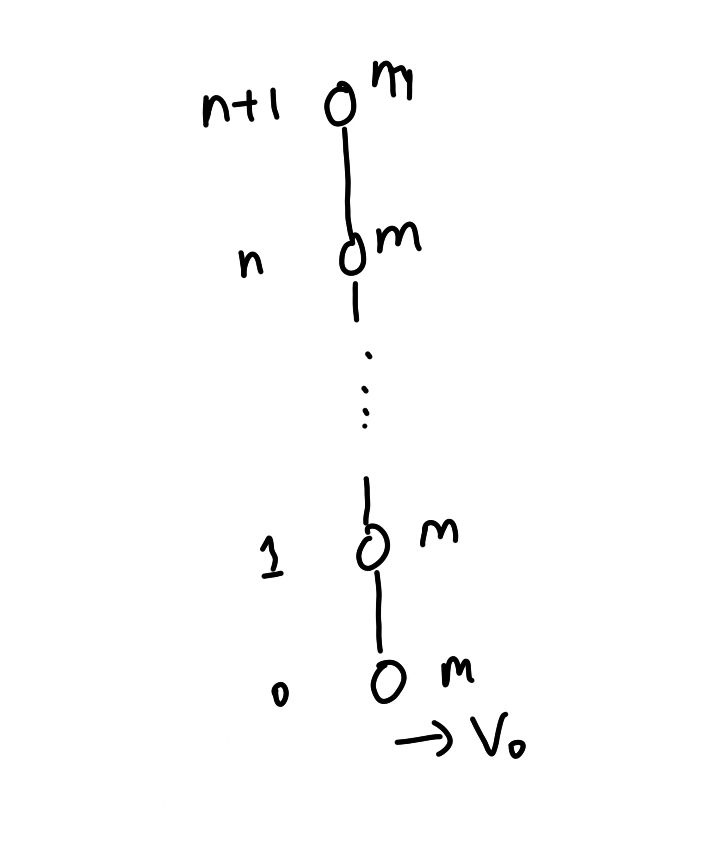
\includegraphics[width=0.3\textwidth]{chainball2}
	\caption{多级链条球.}
	\label{fig:chainball2}
 \end{figure}
\end{enumerate}

\section*{Answer 1}
\begin{enumerate}
	\item 我们设第一根绳子的向右偏离竖直方向的角度为\(\theta_1\),第二根绳子的向右偏离竖直方向的角度为\(\theta_2\),写出系统动能与势能:
	\begin{align*}
		T &= \frac{1}{2}ml^{2}\dot{\theta}_1^2 + \frac{1}{2}ml^{2}(\dot{\theta}_1+\dot{\theta}_2)^2 \\
		V &= -mglcos\theta_1 - mgl(cos\theta_1+cos\theta_2) \\
		  &= V_{0} + mgl(\theta_1^2 + \frac{1}{2}\theta_2^2) 
	\end{align*}
	进而有拉格朗日函数:
	\begin{align*}
		L &= T - V \\
		  &= \frac{1}{2}ml^{2}\dot{\theta}_1^2 + \frac{1}{2}ml^{2}(\dot{\theta}_1+\dot{\theta}_2)^2 - mgl(\theta_1^2 + \frac{1}{2}\theta_2^2) 
	\end{align*}
	对\(\theta_1\)与\(\theta_2\)分别求拉格朗日方程:
	\begin{align*}
		\frac{d}{dt}(\frac{\partial L}{\partial \dot{\theta}_1}) - \frac{\partial L}{\partial \theta_1} &= 0 \\
		\frac{d}{dt}(\frac{\partial L}{\partial \dot{\theta}_2}) - \frac{\partial L}{\partial \theta_2} &= 0 
	\end{align*}
	进而有:
	\begin{align*}
		2mgl\theta_1 + ml^{2}\ddot{\theta}_1 + ml^{2}(\ddot{\theta}_1+\ddot{\theta}_2) &= 0 \\
		mgl\theta_2 + ml^{2}(\ddot{\theta}_1+\ddot{\theta}_2) &= 0 
	\end{align*}
	进而有:
	\begin{align*}
		2\ddot{\theta}_1 + \ddot{\theta}_2 + 2\frac{g}{l}\theta_1 &= 0 \\
		\ddot{\theta}_1 + \ddot{\theta}_2 + \frac{g}{l}\theta_2 &= 0 
	\end{align*}
	令\(w_{0}^2= \frac{g}{l}\), 下面开始计算简正坐标:下式乘以\(\lambda\)加上上式可以得到:
	\begin{align*}
		(2+\lambda)\ddot{\theta}_1 + (1+\lambda)\ddot{\theta}_2 + 2w_{0}^2\theta_1 + \lambda w_{0}^2\theta_2 &= 0 
	\end{align*}
	注意到\(\lambda \neq 0 \) or \(-1\).应有:
	\begin{align*}
		\frac{2+\lambda}{1+\lambda} = \frac{2}{\lambda}
	\end{align*} 
	解的\(\lambda = \pm \sqrt{2}\),回代进而可以找到两个简正坐标:
	\begin{align*}
		q_1 &= \sqrt{2}\theta_1 + \theta_2 \\
		q_2 &= \sqrt{2}\theta_1 - \theta_2 
	\end{align*}
	使得:
	\begin{align*}
		\ddot{q}_1 + \frac{\sqrt{2}}{1+\sqrt{2}}w_{0}^2 q_1 &= 0 \\
		\ddot{q}_2 + \frac{\sqrt{2}}{-1+\sqrt{2}}w_{0}^2 q_2 &= 0 
	\end{align*}
	分别获得了两个简谐振动的频率:
	\begin{align*}
		\omega_1 &= \sqrt{2-\sqrt{2}}w_{0} \\
		\omega_2 &= \sqrt{2+\sqrt{2}}w_{0} 
	\end{align*}
	根据初始条件\(\theta_1=0\), \(\theta_2=0\), \(\dot{\theta}_1=0\), \(\dot{\theta}_2=\frac{v_0}{l}\)可以得到简正坐标的初始条件:
	\begin{align*}
		q_1(0) &= 0 \\ 
		q_2(0) &= 0 \\ 
		\dot{q}_1(0) &= \frac{v_0}{l} \\ 
		\dot{q}_2(0) &= -\frac{v_0}{l} 
	\end{align*}
	进而可以得到简正坐标的解:
	\begin{align*}
		q_1(t) &= \frac{v_0}{\omega_1 l}sin(w_1 t) \\
		q_2(t) &= -\frac{v_0}{\omega_2 l}sin(w_2 t) 
	\end{align*}
	反解得到\(\theta_1(t)\)与\(\theta_2(t)\)的解:
	\begin{align*}
		\theta_1(t) &= \frac{v_0}{2\sqrt{2}l}(\frac{sin(w_1 t)}{w_1} - \frac{sin(w_2 t)}{w_2}) \\
		\theta_1(t) &= \frac{v_0}{2l}(\frac{sin(w_1 t)}{w_1} + \frac{sin(w_2 t)}{w_2}) 
	\end{align*}
	于是下方球体水平方向上的位移为:
	\begin{align*}
		x(t) &= l(\theta_1(t) + \theta_2(t)) \\
		&= \frac{v_0}{2l}((1+\frac{1}{\sqrt{2}}) \frac{sin(w_1 t)}{w_1} + (1-\frac{1}{\sqrt{2}}) \frac{sin(w_2 t)}{w_2}) 
	\end{align*}
	\item 由上式可以看出,由于两个简谐振动的频率为无理数倍,最大值为幅度相加,\(x(t)\)的最大值为:
	\begin{align*}
		x_{max} &= \frac{v_0}{2\sqrt{2}l}((\sqrt{2}+1){w_1} + (\sqrt{2}-1){w_2}) 
	\end{align*}
	\item 首先必须要求同频率,也就是只有一个简正坐标在起作用,这可以通过初始条件来实现:
	例如,通过\(q_2\equiv 0\)来实现。而这也意味着\(\theta_1\)与\(\theta_2\)的初始条件必须满足:
	\begin{align*}
		\sqrt{2}\theta_1(0)-\theta_2(0) &= 0 \\
		\sqrt{2}\dot{\theta}_1(0)-\dot{\theta}_2(0) &= 0 
	\end{align*}
	在已有的限制\(v_{0}= l(\dot{\theta}_1(0)+\dot{\theta}_2(0))\)下,可以计算出来
	\begin{align*}
		\dot{\theta}_1(0) &= \frac{v_0}{l(\sqrt{2}+1)} \\
		\dot{\theta}_2(0) &= \frac{\sqrt{2}v_0}{l(\sqrt{2}+1)}
	\end{align*}
	也就是说,可以让中间球体的初速度为\(\frac{v_0}{\sqrt{2}+1}\),这样就可以实现“更有规律”的摆动。
	或者也可以通过另外一个简正坐标来实现,不难最后得到只需要让中间球体的初速度为\(\frac{v_0}{-\sqrt{2}+1}\)即可。(这种对应向左运动)
	\item 套用前面的结果,我们有再一次回到最低点的时候对应\(\theta_1=0\)
	也就是:
	\begin{align*}
		\frac{sin(w_1 t)}{w_1} - \frac{sin(w_2 t)}{w_2}
		&= 0 
	\end{align*}
	其结果不难由卡西欧得出,设得出的解为\(T\).
	获得此时中间球体的速度为:
	\begin{align*}
		v_{1} &= \frac{v_0}{2\sqrt{2}}(cosw_1 T - cosw_2 T) 
	\end{align*}
	注意到每次都回到最低点的时间是与初速度无关的,结果均为\(T\),于是可以将此速度用于迭代,最后获得编号为\(n\)的球体的速度为:
	\begin{align*}
		v_{n} &= \frac{v_0}{2\sqrt{2}}(cosw_1 T - cosw_2 T)^{n} 
	\end{align*}
	最后可以得到编号为\(n\)的球体的位移为:
	\begin{align*}
		x_{n}(t) &= \frac{v_0}{2\sqrt{2}w_0}(cosw_1 T - cosw_2 T)^{n} sin (w_0 t)
	\end{align*}


\end{enumerate}
\section{Fire !(50pts)}
Naviya在练习她的玫瑰礼花炮弹,她首先测试一下低功率火力的情况,她选择了一块平地作为测试场地。已知重力加速度为\(g\),炮弹的初速度为\(v_{0}\)。
\begin{enumerate}
	\item 如图\ref{fire1} 所示,Naviya发现她的炮弹的轨迹是抛物线,并且无意中发现似乎发射点到抛物线的焦点的距离一直是一个定值,并且还发现抛物线的准线一直没有发生改变,请你帮她证明这现象的正确性。(10pts)
	\begin{figure}[htbp]
	\centering
	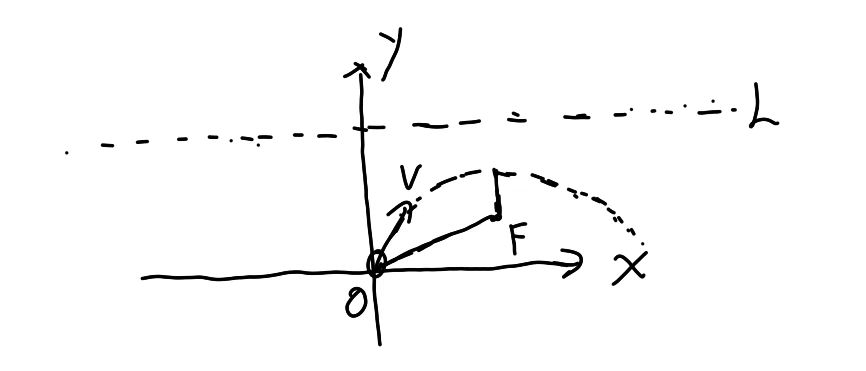
\includegraphics[width=0.5\textwidth]{fire1}
	\caption{炮弹轨迹示意图.}
	\label{fire1}
	\end{figure}
	\item 接着她想测试一下她的范围在限定的速度下能达到的最远的范围,也就是需要求出所有的抛物线的包络线,她猜测包络线也是一个抛物线,也就是对于任意轨迹上的任意一点P,到某一个点的距离始终小于或等于(可以取到等号)到某一条直线的距离。请你帮她找到这个点和这个直线,并且证明她的猜测是正确的,在写出包络线方程。(推荐几何方法解题哦,不过你也可以直接数学解析爆算但可能对下面题没有启发性)(10pts)
	\item 接着她开始加大炮塔的功率,使得炮弹的速度可以飞向太空中,但并没有超过第二宇宙速度。如图\ref{fire2}所示,她发现此时炮弹的轨迹变成了椭圆,她想知道现在发射点到焦点的距离是否还是一个定值?论证你的结论并帮她求出此时能达到的所有范围的包络线方程。(已知万有引力常数为\(G\),地球质量为\(M\),地球半径为\(R\),坐标原点设在地球中心,此问你可以不用考虑地球的碰撞体积)(20pts)
	\item 定义Naviya炮弹最小速度为使得第三问中的包络线恰好与地球表面相切的速度大小,求出这个速度的表达式。(10pts)
	\item 思考题:如果Naviya炮弹的速度超过了第二宇宙速度,那么包络线又会是什么?(0pts)
	\begin{figure}[htbp]
	\centering
	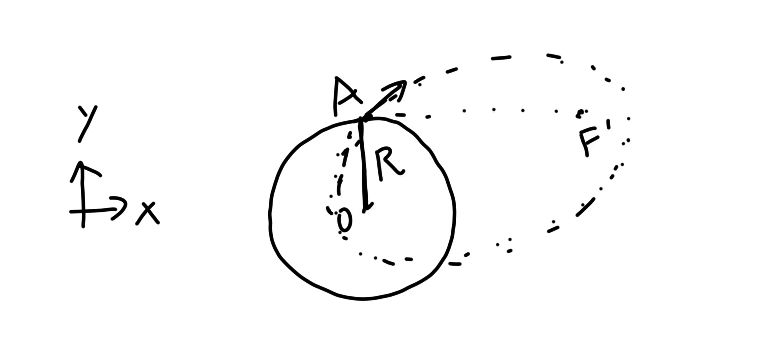
\includegraphics[width=0.5\textwidth]{fire2}
	\caption{炮弹轨迹示意图.}
	\label{fire2}
	\end{figure}
\end{enumerate}

\section*{Answer 2}
\begin{enumerate}
	\item 不难得到当以角度\(\theta\)发射炮弹时,炮弹的运动方程为:
	\begin{align*}
		x(t) &= v_0 \cos \theta t \\
		y(t) &= v_0 \sin \theta t - \frac{1}{2}gt^2
	\end{align*}
	将\(t\)消去,得到抛物线方程为:
	\begin{align*}
		y &= \frac{g}{2v_0^2 \cos^2 \theta} x^2 - \tan \theta x
	\end{align*}
		我们可以看到,抛物线的半正交弦为\(p=\frac{v_0^2 \cos^2 \theta}{g}\), 
		焦点坐标为:
	\begin{align*}
			F_x &= \frac{v_0^2 \sin2 \theta}{2g} \\
			F_y &= -\frac{v_0^2 \cos2 \theta}{2g}
	\end{align*}
	OF的距离为一个定值:
	\begin{align*}
		OF &= \sqrt{F_x^2 + F_y^2} \\
		   &= \frac{v_0^2}{2g} \sqrt{\sin^2 2\theta + \cos^2 2\theta} \\
		   &= \frac{v_0^2}{2g}
	\end{align*}
		而抛物线的准线为:
	\begin{align*}
		y &=h + \frac{p}{2} \\
		h &= \frac{v_0^2 \sin^2 \theta}{2g} \\
		p &= \frac{v_0^2 \cos^2 \theta}{g} \\
		y &= \frac{v_0^2}{2g} 
	\end{align*}
	\item 如图\ref{fire1a}所示,设点\(P\)为抛物线上的任意一点,点\(F\)为焦点,构造一条新的直线\(L_2\),它与抛物线准线的距离恰好为\(\Delta = OF = \frac{v_0^2}{2g}\).
	\begin{figure}[htbp]
	\centering
	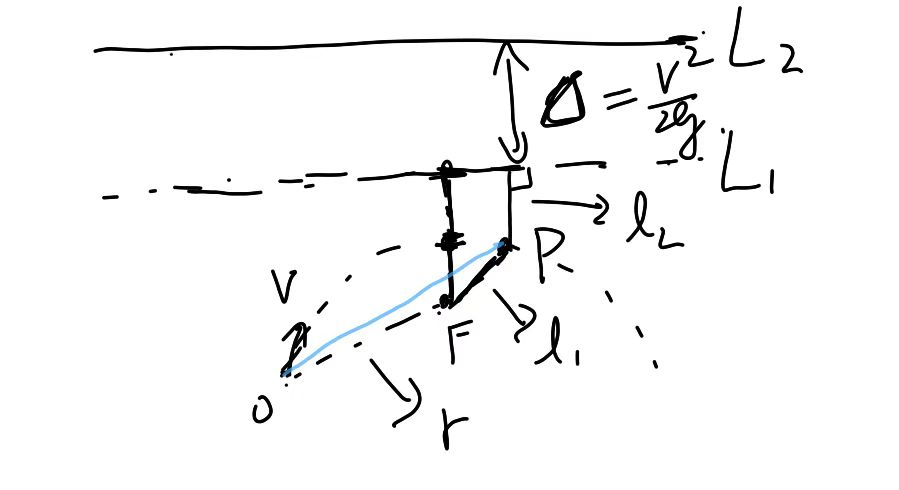
\includegraphics[width=0.5\textwidth]{fire1a}
	\caption{炮弹轨迹示意图.}
	\label{fire1a}
	\end{figure}
		我们可以看到
	\begin{align*}
		OP &\leq OF + l_1=\Delta +l_2 
	\end{align*}
	于是我们看到,OP始终小于等于到\(L_2\)的距离,并且可以取到等号。
		所以包络线就是一条抛物线,焦点为原点O,准线为\(L_2\).对应的\(p'=\Delta=\frac{v_0^2}{2g}\)方程为:
	\begin{align*}
		x^2=-2p'(y-p')  
	\end{align*}
	\item 首先我们计算半长轴\(a\),
	由能量:
	\begin{align*}
		E = \frac{1}{2}mv_0^2 - \frac{GMm}{R} = -\frac{GMm}{2a} \\
		a = -\frac{GM}{2E} = \frac{GMR}{2GM - v_0^2R}
	\end{align*}
	作图如下:
	\begin{figure}[htbp]
	\centering
	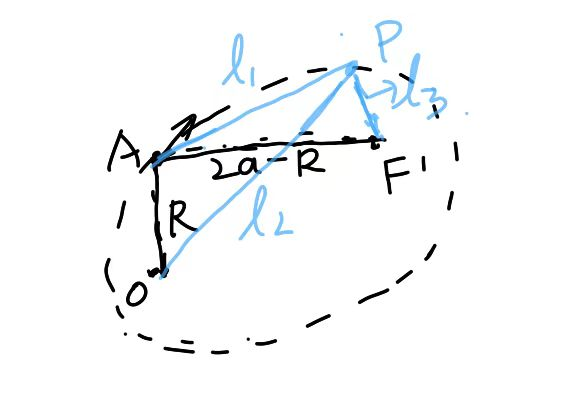
\includegraphics[width=0.5\textwidth]{fire2a}
	\caption{炮弹轨迹示意图.}
	\label{fire2a}
	\end{figure}
		我们可以看到,炮弹的轨迹是一个椭圆,焦点为\(O,F'\),我们有:
	\begin{align*}
		AF' = 2a - R
	\end{align*}
	也为一个定值!(这也说明椭圆的另一个焦点的轨迹是一个圆,但这一点性质并没有什么用。)我们又有\(l_2+l_3=2a\),
	从而:
	\begin{align*}
		l_1+l_2\leq  (AF' + l_3) + l_2 = AF' + 2a = 4a - R
	\end{align*}
	恒小于等于一个定值,并且可以取到等号。
		所以包络线就是一条椭圆,焦点为\(O,A\),半长轴为\(A=2a-\frac{R}{2}\),半焦距为\(C=\frac{R}{2}\),半短轴为\(B=\sqrt{a^2-c^2}\),注意坐标原点为O, 故Naviya包络线方程为:
	\begin{align*}
		\frac{x^2}{(2a-\frac{R}{2})^2} + \frac{(y-\frac{R}{2})^2}{(2a-\frac{R}{2})^2-(\frac{R}{2})^2} = 1
	\end{align*}
	\item 与地球方程联立:
	\begin{align*}
		\frac{x^2}{(2a-\frac{R}{2})^2} + \frac{(y-\frac{R}{2})^2}{(2a-\frac{R}{2})^2-(\frac{R}{2})^2}  &= 1 \\
		x^2 + y^2 &= R^2
	\end{align*}
	消去\(x\),令\(Y=\frac{y}{R}\),\(\lambda = \frac{A}{R}\),我们有:
	\begin{align*}
		Y^2 -4Y\lambda^2+2\lambda^2-1 &= 0 
	\end{align*}
	要求相切,则要求只能恰好有一个\(Y\)的解,判别式为:
	\begin{align*}
		\Delta &= 16\lambda^4 - 8\lambda^2 + 4 =0
	\end{align*}
		我们可以得到:
	\begin{align*}
		\lambda = \frac{\sqrt{1+\sqrt{5}}}{2}
	\end{align*}
	于是我们可以得到Naviya炮弹的最小速度为:
	\begin{align*}
		a &= \frac{1+\sqrt{1+\sqrt{5}}}{4}R \\
		v_{Naviya} &= \sqrt{\frac{GM}{R}(2-\frac{4}{1+\sqrt{1+\sqrt{5}}})} 
	\end{align*}

\end{enumerate}
\section{碰 (40pts)}
瓦雷莎正在锻炼她的碰撞本领,她会去尝试冲撞一个静止的巨石。下面让我们来帮她分析一下情况,我们将他们抽象为两个质点,分别为\(m_1\)和\(m_2\),其中\(m_1\)为瓦雷莎,\(m_2\)为静止的巨石。瓦雷莎以初始动量\(p_0\)向右冲撞巨石,考虑相对论效应,已知光速为\(c\),则瓦雷莎初始能量为\(E_1 = \sqrt{p_0^2c^2 + m_1^2c^4}\)。如图\ref{peng1} 所示:
\begin{figure}[htbp]
	\centering
	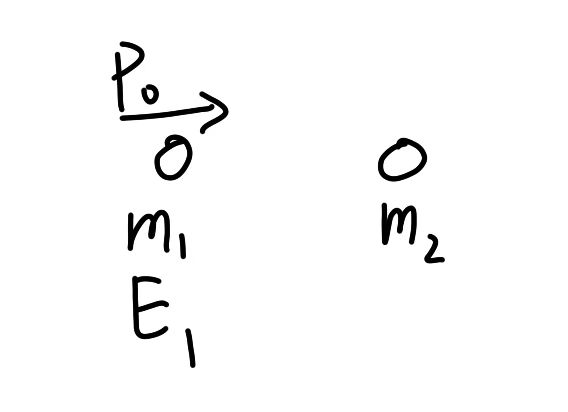
\includegraphics[width=0.3\textwidth]{peng1}
	\caption{碰撞示意图.}
	\label{peng1}
\end{figure}
\begin{enumerate}
	\item 我们先为这个分析打一个基础:已知空间中有\(n\)个质点,它们的动量分别为\(\vec{p}_1,\vec{p}_2,\cdots,\vec{p}_n\),能量分别为\(E_1,E_2,\cdots,E_n\),请你证明:存在一个参考系,它相对于当前参考系的速度为\(\vec{\beta}_c c\), 使得在这个参考系中,所有的质点的总动量为0,并求出\(\vec{\beta}_c\)的表达式。(12pts)
	\item 现在回来分析瓦雷莎的情况,请问什么情况下她会直接被巨石原路反弹?请给出条件,当不会反弹时,求出她的最大可能的偏离原来方向的角度。(28pts)
\end{enumerate}

\section*{Answer 3}
\begin{enumerate}
	\item 首先我们在实验系下找一个方向使得在这个方向上的总动量为0(这必然找得到,因为总动量是一个矢量,必然可以旋转坐标架做到这一点), 设这个方向为\(y\)轴,\(x\)轴为垂直于\(y\)轴的方向。现在令\(\beta_c\)方向沿着\(x\)轴,有:
	\begin{align*}
		\sum_{i=1}^{n} p_{i,y}' &= \sum_{i=1}^{n} p_{i,y}= 0 \\
		\sum_{i=1}^{n} p_{i,x}' &= \sum_{i=1}^{n} \gamma_c (p_{i,x} - \beta_c \frac{E_{i}}{c}) = 0 
	\end{align*}
	于是解的\(\beta_c\)为:
	\begin{align*}
		\beta_c &= \frac{\sum_{i=1}^{n} p_{i,x}c}{\sum_{i=1}^{n} E_{i}} 
	\end{align*}
	注意到所选轴的特殊性,有:
	\begin{align*}
		\vec{\beta}_c &= \frac{\sum_{i=1}^{n} \vec{p}_{i}c}{\sum_{i=1}^{n} E_{i}} 
	\end{align*}
	现在完全变成了矢量形式,与坐标架的选择无关了,证毕。
	\item 我们换到零动量系,也就是\(\vec{\beta}_c = \frac{\vec{p}_0 }{E_1 + m_2c^2}\),在这个系下,二者的动量大小相等方向相反,设大小为\(p'\), 有:
	\begin{align*}
		p' &= \gamma_c (p_0- \beta_c \frac{E_{1}}{c}) = \gamma_c \beta_c m_2 c \\
		E_1' &= \sqrt{p'^2c^2 + m_1^2c^4} = \gamma_c (E_1 -\beta_c p_0 c)\\
		E_2' &= \sqrt{p'^2c^2 + m_2^2c^4}
	\end{align*}
	在这个参考系下,碰撞前后的能量守恒与动量守恒会保证二者的动量大小相等方向相反,且大小仍为\(p'\)。(因为这里的解是唯一的,有两个方程。)唯一不同的只有方向,设偏向的角度为\(\theta\),将动量变换回去,得到:
	\begin{align*}
		p_{1,x} &= \gamma_c ( p' \cos \theta + \beta_c \frac{E_{1}'}{c}) \\
		p_{1,y} &= p' \sin \theta  
	\end{align*}
	因此,如果出现反弹的情况,必然有\(\theta = \pi\)时\(p_{1,x} < 0\), 也就是:
	\begin{align*}
		\frac{\beta_c E_1'}{p' c} < 1
	\end{align*}
	化简得:
	\begin{align*}
		\frac{E_1 m_2 + m_1^2 c^4}{E_1 m_2+ m_2^2 c^4} < 1 
	\end{align*}
	这也意味着:
	\begin{align*}
		m_1 < m_2
	\end{align*}
	所以只要瓦雷莎的质量大于巨石的质量,她就会不会被反弹。否则她会被反弹。当不会被反弹时:
	\begin{align*}
		tan\theta &= \frac{p_{1,y}}{p_{1,x}} = \frac{p' \sin \theta}{\gamma_c ( p' \cos \theta + \beta_c \frac{E_{1}'}{c})} 
	\end{align*}
	对上式求导令其为0,得到:
	\begin{align*}
		cos\theta = -\frac{p' c}{\beta_c E_1'} = -\frac{E_1 m_2 + m_2^2 c^4}{E_1 m_2+ m_1^2 c^4}
	\end{align*}
	可见也是只有在\(m_1 > m_2\)时,才有解。回代,得到:
	\begin{align*}
		tan\theta &= \frac{1}{\gamma_c \sqrt{(\frac{\beta_c E_1'}{p' c})^2-1}} 
	\end{align*}
	最终的结果为:
	\begin{align*}
		\theta &= \arctan \left(\frac{1}{\sqrt{1-(\frac{p_0}{E_1 + m_2c^2})^2}\sqrt{(\frac{E_1 m_2 + m_1^2 c^4}{E_1 m_2+ m_2^2 c^4})^2-1}} \right)
	\end{align*}

\end{enumerate}
\section{地脉热管(50pts)}
近日,Teyvat地脉深处发生了一系列紊乱,导致地脉热管的异常升温。这些热管是连接地脉与地表的重要通道,它们的温度升高可能会引发一系列地质灾害。地脉流动着许多的熔岩物质,这些熔岩的密度为\(\rho(\vec{r},t)\),单位质量的热容为\(c\),流速为\(\vec{v}(\vec{r},t)\),流动的熔岩在地脉中具有许许多多的热量交换。已知傅里叶定律为:\(\vec{j}_c = -k \nabla T\)。为单位时间单位面积内传导的热量,\(k\)为导热系数,为常数。下面你均只需要考虑热传导和热对流,不考虑其他因素的影响。
\begin{enumerate}
	\item 已知地脉中的温度分布为\(T(\vec{r},t)\),请你推导出地脉中熔岩的热量流动方程,即关于温度\(T(\vec{r},t)\)的方程(5pts)
	\item 现在考虑连接地脉与地表的热管,为简单起见,我们将热管视为一个圆柱体,半径为\(R\),长度为\(L\),底面与地脉的接触面积为\(S\),热管底部与顶部的温度分别为\(T_1\), \(T_2\),假设热管熔岩中的温度分布已经达到了稳态,并假设热管中的熔岩流速为常数向上的\(v\),并设热管具有散热功能,单位时间单位面积散热量为\(\alpha T\),请你推导出热管中熔岩的温度分布\(T(x)\),\(x\)为沿着热管的轴向坐标,从下至上为\(0\)到\(L\)。(30pts)
	\item 并求出该热管的总散热量\(Q_c\)。(10pts)
	\item 现在考虑一个二维的流动着的稳态柱对称的熔岩,其流速径向向外流动\(v(r)\),设原点有源源不断的熔岩流出,流量为\(Q\),请你推导出熔岩的温度分布\(T(r)\)满足的微分方程。(5pts)
\end{enumerate}

\section*{Answer 4}
\begin{enumerate}
	\item 空间中的热流为:
	\begin{align*}
		\vec{j} = \vec{j}_c + \vec{j}_d = -k \nabla T + \rho c T\vec{v} 
	\end{align*}
	做一个高斯面积分,得到:
	\begin{align*}
		\frac{\partial}{\partial t} \int_V \rho c T dV + \int_S \vec{j} \cdot dS = 0
	\end{align*}
		根据高斯定理,有:
	\begin{align*}
		\int_S \vec{j} \cdot dS = \int_V \nabla \cdot \vec{j} dV
	\end{align*}
		因此有:
	\begin{align*}
		\frac{\partial (\rho c T)}{\partial t} = k \nabla^2 T -  \nabla \cdot(\rho c T\vec{v})
	\end{align*}
		
	\item 设热管中熔岩的温度分布为\(T(x)\),则根据稳态条件,有:
	\begin{align*}
		j(x) &= -k \frac{\partial T}{\partial x} + \rho c v T(x) \\
		j'(x)S &= -2\pi R \alpha T(x) 
	\end{align*}
	整理得到微分方程为:
	\begin{align*}
		-kS T''(x) + \rho cS v T'(x) = -2\pi R \alpha T(x)
	\end{align*}
	两个特征根为:
	\begin{align*}
		\lambda_{1,2} &= \frac{\rho c v}{2k} \pm \sqrt{(\frac{\rho c v}{2k})^2 + \frac{2\pi R \alpha}{kS}}
	\end{align*}
		因此通解为:
	\begin{align*}
		T(x) &= A e^{\lambda_1 x} + B e^{\lambda_2 x} \\
		j(x) &= -k \frac{\partial T}{\partial x} + \rho c v T(x)
	\end{align*}
	带入边界条件:
	\begin{align*}
		T(0) &= T_1 \\
		T(L) &= T_2
	\end{align*}
		得到:
	\begin{align*}
		A &= \frac{T_2 - T_1 e^{\lambda_2 L}}{e^{\lambda_1 L} - e^{\lambda_2 L}} \\
		B &= \frac{T_1 e^{\lambda_1 L} - T_2 }{e^{\lambda_1 L} - e^{\lambda_2 L}}
	\end{align*}
		热管的总散热量为:
	\begin{align*}
		Q_c &= j(0)S-j(L)S \\
		&= [-kS \frac{\partial T(x)}{\partial x} + \rho c Sv T(x)]_{0}^L \\
		&= AS(e^{\lambda_1 L} - 1)(-k\lambda_1+c\rho v) + BS(e^{\lambda_2 L} - 1)(-k\lambda_2+c\rho v) 
	\end{align*}
	\item 先求流速的表达式:
	\begin{align*}
		Q &= 2\pi R v(r) \\
		v(r) &= \frac{Q}{2\pi r}
	\end{align*}
	带入(1)的方程,得到:
	\begin{align*}
		 k T''(r) -  \frac{Q\rho c}{2\pi } \frac{d}{d r} (\frac{T(r)}{r})=0\\
	\end{align*}



\end{enumerate}
\section{镜 (45pts)}
如图\ref{mirror} 所示,这道题是三个简单的几何光学问题。所有镜子的距离是\(d\),焦距是\(f\)或者\(-f\),设第一个物距为\(u\),请你回答下面的问题:
\begin{figure}[htbp]
	\centering
	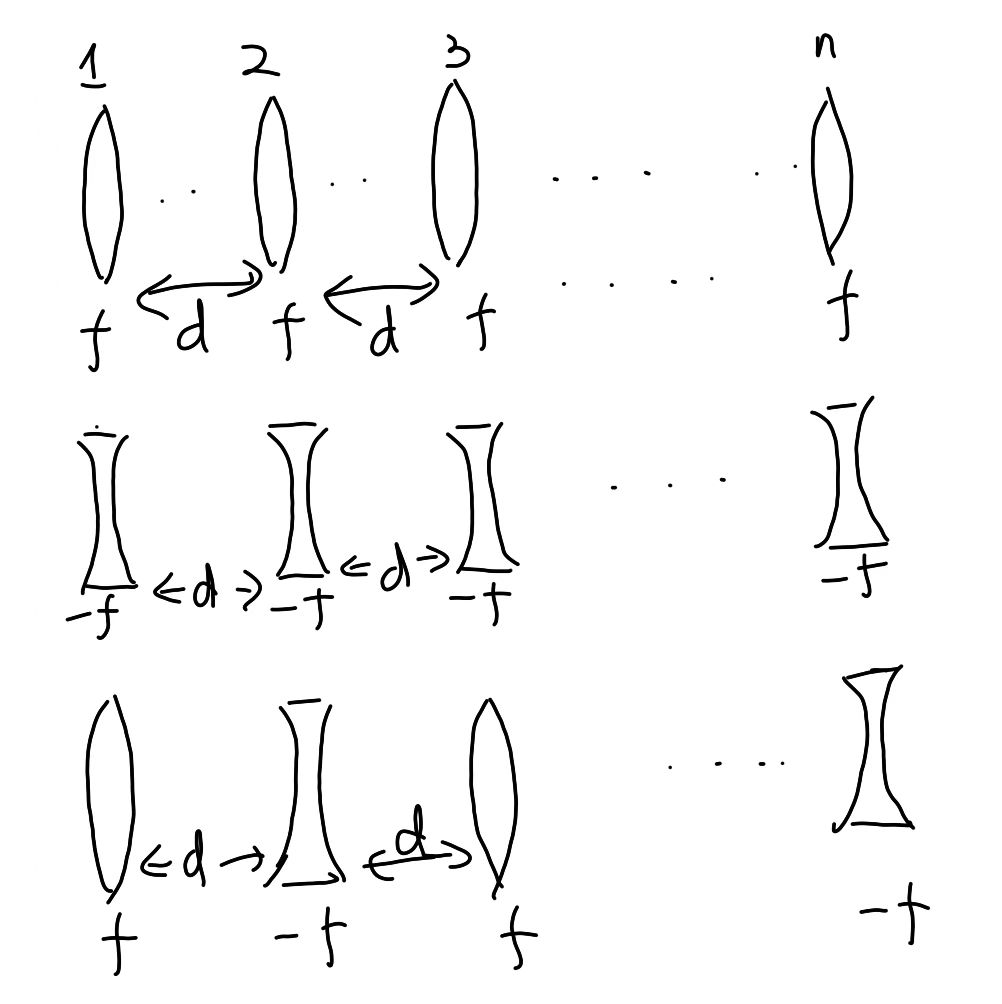
\includegraphics[width=0.5\textwidth]{mirror}
	\caption{这是三道摆放方案.}
	\label{mirror}
\end{figure}
\begin{enumerate}
	\item 光路全由凸透镜构成,总共\(n\)个凸透镜,求出最后的像距\(v\)与物距\(u\)的关系式。提示:你需要分两种情况讨论:\(d=4f\), \(d\neq 4f\)。 (30pts)
	\item 光路全由凹透镜构成,总共\(n\)个凹透镜,求出最后的像距\(v\)与物距\(u\)的关系式。(5pts)
	\item 光路全由凹透镜和凸透镜交替构成,总共\(n\)个透镜,得出相邻两项递推关系式给出计算方法即可(需要确保可以实现),无需给出具体答案(10pts) 
\end{enumerate}

\section*{Answer 5}
\begin{enumerate}
	\item 有成像公式:
	\begin{align*}
		\frac{1}{f} &= \frac{1}{u} + \frac{1}{v} \\
		v &= \frac{fu}{u-f}\\
		u_{n} & = d-v_n \\
		v_n &= \frac{fu_{n}}{u_{n}-f} 
	\end{align*}
	可以填充定义:
	\begin{align*}
		v_0 = d - u
	\end{align*}
	递推关系为:
	\begin{align*}
		v_{n+1} &= \frac{(d-v_n)f}{d-v_n-f} 
	\end{align*}
	使用不动点法,令\(v_{n+1} = v_n = x\),得到:
	\begin{align*}
		x^2 -  xd + fd &= 0 
	\end{align*}
	当\(d=4f\)的时候,只有一个解:
	\begin{align*}
		x = \frac{d}{2} = 2f
	\end{align*}
	此时我们做一下数学变换:
	\begin{align*}
		v_{n+1} - 2f &= \frac{v_n - 2f}{3f - v_n}f \\
		\frac{f}{v_{n+1} - 2f} &= \frac{3f - v_n}{v_n - 2f} = \frac{f}{v_n - 2f} - 1 
	\end{align*}
	发现为等差数列,立即递推得出:
	\begin{align*}
		\frac{f}{v_{n} - 2f} &= \frac{f}{v_0 -2f} - n 
	\end{align*}
	由此可得:
	\begin{align*}
		v = v_n = 2f + \frac{f}{\frac{f}{2f - u} - n} 
	\end{align*}
	当\(d \neq 4f\)的时候,有两个解(不论是实数还是复数均可以):
	\begin{align*}
		&x_1 x_2 = fd \\
		&x_1 + x_2 = d 
	\end{align*}
	对递推关系做变换:
	\begin{align*}
		v_{n+1} -x_1 &= \frac{(d-v_n)f}{d-v_n-f} - x_1 \\
		&= \frac{df - v_n f - x_1 d - v_n x_1 - f x_1}{d-v_n-f} \\
		&= \frac{(v_1 - x_1 )(x_1 -f )}{d-v_n-f} \\
		v_{n+1} - x_2 &= \frac{(v_1 - x_2 )(x_2 -f )}{d-v_n-f} \\
	\end{align*}
	两式相除,得到:
	\begin{align*}
		\frac{v_{n+1} - x_1}{v_{n+1} - x_2} &= \frac{(v_n - x_1 )(x_1 -f )}{(v_n - x_2 )(x_2 -f )} 
	\end{align*}
	发现为等比数列,于是立即递推得出:
	\begin{align*}
		\frac{v_{n} - x_1}{v_{n} - x_2} &= \frac{v_0 - x_1}{v_0 - x_2} \prod_{i=0}^{n-1} \frac{x_1 -f}{x_2 -f} \\
		&= \frac{v_0 - x_1}{v_0 - x_2} \left(\frac{x_1 -f}{x_2 -f}\right)^n 
	\end{align*}
	从而得到:
	\begin{align*}
		v_n &=\frac{x_1 + \frac{v_0 - x_1}{v_0 - x_2} \left(\frac{x_1 -f}{x_2 -f}\right)^n x_2}{1+ \frac{v_0 - x_1}{v_0 - x_2} \left(\frac{x_1 -f}{x_2 -f}\right)^n} 
	\end{align*}
	带入\(v=v_n, v_0 = d-u\),得到:
	\begin{align*}
		v &= \frac{x_1 + \frac{d-u - x_1}{d-u - x_2} \left(\frac{x_1 -f}{x_2 -f}\right)^n x_2}{1+ \frac{d-u - x_1}{d-u - x_2} \left(\frac{x_1 -f}{x_2 -f}\right)^n} 
	\end{align*}
	\item 这里注意到只需要将\(f\)换成\(-f\)即可,并且注意到了此时将不会有分类讨论的情况,因为距离永远是大于0的。
	\begin{align*}
		v &= \frac{x_1 + \frac{d-u - x_1}{d-u - x_2} \left(\frac{x_1 +f}{x_2 +f}\right)^n x_2}{1+ \frac{d-u - x_1}{d-u - x_2} \left(\frac{x_1 +f}{x_2 +f}\right)^n} 
	\end{align*}
	\item 此时我们仍从递推关系出发:(令\(v_0 = d-u\))
	\begin{align*}
		\frac{1}{d-v_0} + \frac{1}{v_1} &= \frac{1}{f} \\
		\frac{1}{d-v_1} + \frac{1}{v_2} &= \frac{1}{-f}
	\end{align*}
	此时的相邻的递推需要是角标差为2的关系式:
	\begin{align*}
		v_2 = \frac{(d^2 - 2df + (f-d)v_0)(-f)}{d^2-df-f^2-dv_0}
	\end{align*}
	不难发现我们仍然可以使用不动点发做,然后同第一小问一样的解法即可。

\end{enumerate}
\section{开关?电阻?(40pts)}
Nahida发现了一个古老的须弥电路图,如图\ref{switch} 所示,她想一会后意识到这个具有把开关当成电阻的功能。请你也来学习一下她的芝士吧!
\begin{figure}[htbp]
	\centering
	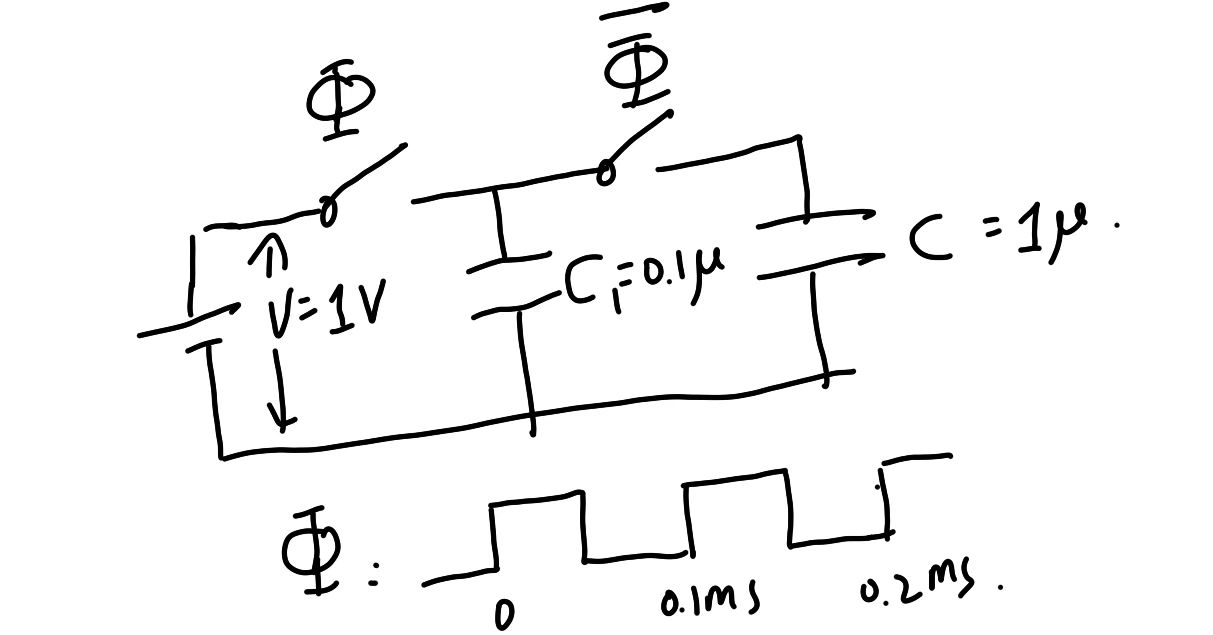
\includegraphics[width=0.5\textwidth]{switch}
	\caption{这是一个简单的电路图.}
	\label{switch}
\end{figure}
\begin{figure}[htbp]
	\centering
	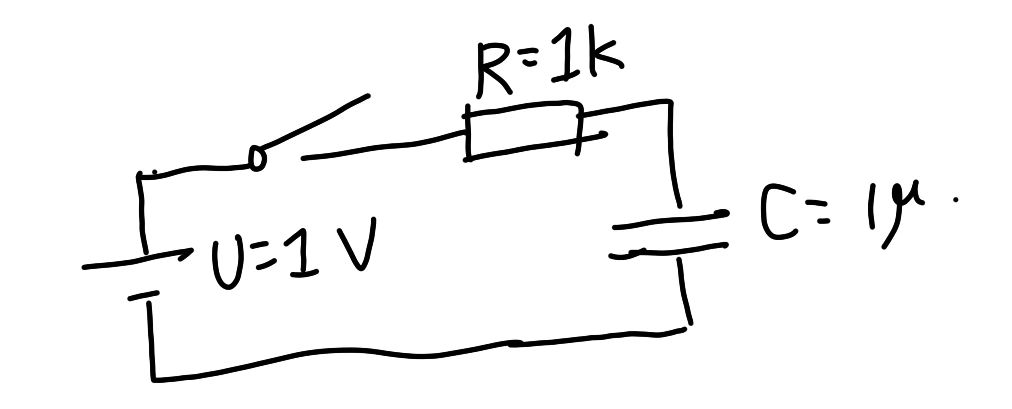
\includegraphics[width=0.5\textwidth]{RC}
	\caption{这真的是一个简单的电路图.}
	\label{RC}
\end{figure}
\begin{enumerate}
	\item 请求出图\ref{RC} 中的电容电压随时间的变化关系式\(V_c(t)\) (4pts)
	\item 请求出图\ref{switch} 中的电容电压随时间的变化关系式\(V_c'(t)\)。图示中有两个开关(cmos管)受到信号\(\Phi\)的控制,两个开关的信号恰好相反,只有当高电平的时候开关才会闭合。 硬件参数已经如图所示(24pts)
	\item 请给出若要把图示的开关完全等效为一个电阻\(R\)的条件,并且与原本的电容\(C\)无关。(12pts)
\end{enumerate}

\section*{Answer 6}
\begin{enumerate}
	\item 由电容充电公式可得:
	\begin{align*}
		V_c(t) &= V_0(1-e^{-t/RC}) 
	\end{align*}
	\item 不妨令\(T=0.1ms\),由于没有电阻,每一次都是速充。
	第一个T之后:
	\begin{align*}
		V_c'^{(1)} &= \frac{C_1}{C_1 + C} = \frac{1}{11} V
	\end{align*}
	在\(t=nT\),类推得到:
	\begin{align*}
		V_{c1}^{(n)}=V_c'^{(n)} &= \frac{C_1 +CV_{c1}^{(n-1)}}{C_1 + C}
	\end{align*}
	构造等比数列:
	\begin{align*}
		V_c^{(n)} - 1 = \frac{10}{11} (V_c^{(n-1)} - 1)
	\end{align*}
	\begin{align*}
		V_c^{(n)}=1- \left(\frac{10}{11}\right)^n
	\end{align*}
	加入取整函数得到:
	\begin{align*}
		V_c(t)=1- \left(\frac{10}{11}\right)^{[\frac{t}{T} + \frac{1}{2}]}
	\end{align*}
	\item 不难发现当\(T<<1,t>>T\)时,
	\begin{align*}
		V_c(t)=1- \left(\frac{10}{11}\right)^{[\frac{t}{T} + \frac{1}{2}]}\approx 1- e^{\ln(\frac{10}{11}) \frac{t}{T}}
	\end{align*}
	十分趋近于RC电路的充电公式了。如果在仔细观察一下的话,
	条件应该是:
	\begin{align*}
		\frac{1}{T}\ln(\frac{C_1+C}{C}) = \frac{1}{RC}
	\end{align*}
	当\(C_1<<C\)的时候,就有:
	\begin{align*}
		R \approx \frac{T}{C_1}
	\end{align*}
	此时电阻将于原本的电容大小无关了!这意味着我们可以用电容和开关转换成电阻,这在实际的数字电路中十分常见。


\end{enumerate}
\section{Euler Method (35pts)}
弹簧-质量模型是一个简单的物理系统,由连接到弹簧上的质量组成。质量可以来回移动,这是由弹簧根据胡克定律施加的恢复力引起的。这是一个可以通过数值方法模拟的经典力学系统。\\
质量为$m$的物体连接到弹性常数为$k$的弹簧上的基本运动方程为:
\[
m \frac{d^2x}{dt^2} + kx = 0
\]
这个方程是一个二阶微分方程,我们可以使用数值方法来近似求解这个方程。为此,我们需要离散化时间并用有限差分代替连续导数。我们将考虑求解这类微分方程的两种常见方法:\textbf{显式欧拉法}和\textbf{隐式欧拉法}。
\subsection*{显式欧拉法}
显式欧拉法是近似求解的最简单方法之一。为了应用它,我们需要离散化速度和位置。设$v(t)$为速度,因此:
\[
v(t) = \frac{dx}{dt}, \quad a(t) = \frac{dv}{dt} = \frac{d^2x}{dt^2}
\]
离散时间步骤表示为$t_n = n \Delta t$,其中$\Delta t$是时间步长。使用显式欧拉法:
\begin{itemize}
	\item 位置更新:$x_{n+1} = x_n + v_n \Delta t$;    速度更新:$v_{n+1} = v_n + a_n \Delta t$
\end{itemize}
\subsection*{隐式欧拉法}
隐式欧拉法比显式方法更稳定,尤其是对于刚性系统。它使用下一时间步的值,而不是当前时间步的值来计算更新。隐式欧拉法更新位置和速度如下:
\begin{itemize}
	\item 位置更新:$x_{n+1} = x_n + v_{n+1} \Delta t$;    速度更新:$v_{n+1} = v_n + a_{n+1} \Delta t$
\end{itemize}
设$s_n = [x_n, v_n]$,$s_0 = [x_0, v_0]$为初始状态。
\begin{enumerate}
	\item 基于胡克定律使用$x_n$定义$a_n$。(5pts)
	\item 推导使用显式欧拉法的$\{s_n\}$的通用公式.(20pts)
	\item 推导使用隐式欧拉法的$\{s_n\}$的通用公式.(10pts)
	\item (思考题)解释为什么"隐式欧拉法比显式方法更稳定"。隐式欧拉法可能有哪些缺点?(bonus: 0pts)
\end{enumerate}

\section*{Answer 7}
\begin{enumerate}
	\item 根据胡克定律,$F=-kx=ma$,因此
		\[
			a_n = -\frac{k\,x_n}{m}.
		\]
	\item 我们可以将显式欧拉法写成矩阵形式:
		\[
			\begin{bmatrix}x_{n+1}\\v_{n+1}\end{bmatrix}
			=
			\begin{bmatrix}
				1 & \Delta t\\
				-\tfrac{k}{m}\,\Delta t & 1
			\end{bmatrix}
			\begin{bmatrix}x_n\\v_n\end{bmatrix}
			=
			\begin{bmatrix}
				1 & \Delta t\\
				-\tfrac{k}{m}\,\Delta t & 1
			\end{bmatrix}^{n+1}
			\begin{bmatrix}x_0\\v_0\end{bmatrix}.
		\]
		计算该矩阵的特征值,得到
		\[
			\lambda_{1} = 1 + i\omega\Delta t,\quad
			\lambda_{2} = 1 - i\omega\Delta t,\quad
			\omega = \sqrt{\tfrac{k}{m}}.
		\]
		对应的特征向量为
		\[
			p_{1} = \begin{bmatrix}1\\i\omega\Delta t\end{bmatrix},\quad
			p_{2} = \begin{bmatrix}1\\-i\omega\Delta t\end{bmatrix}.
		\]
		对矩阵进行对角化,可得
		\[
			\begin{bmatrix}x_{n}\\v_{n}\end{bmatrix}
			=
			(1+(\omega\Delta t)^2)^{\frac n2}
			\begin{bmatrix}
				\cos\bigl(n\arctan(\omega\Delta t)\bigr) &
				\tfrac1\omega\sin\bigl(n\arctan(\omega\Delta t)\bigr)\\
				-\omega\sin\bigl(n\arctan(\omega\Delta t)\bigr) &
				\cos\bigl(n\arctan(\omega\Delta t)\bigr)
			\end{bmatrix}
			\begin{bmatrix}x_0\\v_0\end{bmatrix}.
		\]
	\item 对于隐式欧拉法,有
		\[
			\begin{bmatrix}x_{n}\\v_{n}\end{bmatrix}
			=
			\begin{bmatrix}
				1 & -\Delta t\\
				\tfrac{k}{m}\,\Delta t & 1
			\end{bmatrix}
			\begin{bmatrix}x_{n+1}\\v_{n+1}\end{bmatrix}
			=
			\frac1{1+\tfrac{k}{m}\Delta t^2}
			\begin{bmatrix}
				1 & \Delta t\\
				-\tfrac{k}{m}\,\Delta t & 1
			\end{bmatrix}
			\begin{bmatrix}x_{n-1}\\v_{n-1}\end{bmatrix}.
		\]
		同样地,我们对该矩阵计算特征值和特征向量,可得
		\[
			\begin{bmatrix}x_{n}\\v_{n}\end{bmatrix}
			=
			\frac1{(1+\tfrac{k}{m}\Delta t^2)^{\frac n2}}
			\begin{bmatrix}
				\cos\bigl(n\arctan(\omega\Delta t)\bigr) &
				\tfrac1\omega\sin\bigl(n\arctan(\omega\Delta t)\bigr)\\
				-\omega\sin\bigl(n\arctan(\omega\Delta t)\bigr) &
				\cos\bigl(n\arctan(\omega\Delta t)\bigr)
			\end{bmatrix}
			\begin{bmatrix}x_0\\v_0\end{bmatrix}.
		\]
	\item Furina!
\end{enumerate}




\end{document}